\section{分裂法与全分离法}
\label{sec:2.4}
通常同时起作用的两个过程A与B也许是或者
也许不是相互联系的。它们相互独立的这种情形, 称作全分离(full separation)
。在这种情形下,就概念和就计算而言,想像A过程在B过程开始之
前正趋近于结束,这往往是很有用的。在两种过程
彼此有相互联系的场合,有可能是允许A短暂起作
用,然后转换为B起作用,并如此交替作用下去,
这种交替起作用的办法称作分裂法(splitting)。

\subsection{热流方程}
\label{sec:2.4.1}
绕射方程或偏移方程可称作“波阵面恢复”方程,它把初始条件或透镜项可能引起的波阵面的任
何横向突变一起加以平滑恢复原状。
15°偏移方程具有有与热流方程相同的数学形式。不过热
流方程全是实数,而且它的物理性态更容易理解,这点值得多说两句:(l)x方向的热流
$H_x$等于温度的负梯度$-\partial T/\partial x$如乘以热传导率$\sigma$。(2)温度降低$-\partial T/\partial t$是同热流发散量$\partial H_x/\partial x$
除以热容量c成比例。将上述二者结合起来并由一维情形推广至二维情形,取$\sigma$为常数及
$c=l$,得出方程:
\begin{equation}
\frac{\partial T}{\partial t}=\sigma[\frac{\partial^2}{\partial x^2}+\frac{\partial^2}{\partial y^2}]T
\label{eq:ex2.4.1}
\end{equation}

\subsection{分裂法}
\label{sec:2.4.2}
应用于热流方程数值解法的分裂法是用两个微分方程代替热流方程,按交替的时间步长
应用其中每个方程
\begin{subequations}
\begin{equation}
\frac{\partial T}{\partial t}=2\sigma\frac{\partial^2 T}{\partial x^2} \quad (all\quad y)
\label{eq:ex2.4.2a}
\end{equation}
\begin{equation}
\frac{\partial T}{\partial t}=2\sigma\frac{\partial^2 T}{\partial y^2} \quad (all\quad x)
\label{eq:ex2.4.2b}
\end{equation}
\label{eq:ex2.4.2}
\end{subequations}

式\ref{eq:ex2.4.2a}中,对于x方向的热流其热传导率$\sigma$业已增大两倍,而对$y$方向的热流则已取$\sigma$
为零;在式\ref{eq:ex2.4.2b}中,则情形反之。在时间的奇数时刻,热量按式\ref{eq:ex2.4.2a}的关系流
动;在时间的偶数时刻则按式\ref{eq:ex2.4.2b}的关系流动。这种轮流交替采用式\ref{eq:ex2.4.2a}与
\ref{eq:ex2.4.2b}所得的解在数学上可证明是收敛于式\ref{eq:ex2.4.1}的解,其误差为$\Delta t$数量级,因此
汾趋于零时,误差亦趋于零。高维隐式方法的不可行性是促使采用分离法的原因(参阅\ref{sec:2.2}
节结尾部分)。

\subsection{全分离法}
\label{sec:2.4.3}
最终可证明分裂法比可能想像的要精确得多,在许多情形下不存在精度损失。此外,可
认为这种方法是一种极限情形。试考虑一下处理方程\ref{eq:ex2.4.2a}与\ref{eq:ex2.4.2b}的基本方
法,在这种处理中,不是按交错的时间步长在它们之间轮流进行前向与后向计算,而是通过
所有时间步长将方程\ref{eq:ex2.4.2a}计算到底,然后再将这种中间计算结果作为方程\ref{eq:ex2.4.2b}
的初始条件,经过所有时间步长将式\ref{eq:ex2.4.2b}计算到底,得出最终结果。也许会令人惊
奇,这种经过基本改变的方法可以产生方程\ref{eq:ex2.4.1}的正确解。但是,只在$\sigma$是$x$与$y$的一个恒定
函数时,才能如此。对于脉冲型初始扰动的情形,该种过程如图\ref{fig:txz/temperature}所示。在用这种基本
方法获得正确的解时,就把像\ref{eq:ex2.4.1}那样的一种微分方程说成是可全分离的。全分离法
在$\sigma$为常数时才有效,这点不应使人感到太奇怪,因为这时才能够应用Fourier变换,从而
二维解$exp[-\sigma(k_x^2+k_y^2)t]$等于一维解$exp(-\sigma k_x^2t)$与$exp(-\sigma k_y^2t)$之乘积。可以证明
并且以后将会指出,可应用全分离法的条件就是$\sigma \partial^2/\partial x^2$应能与$\sigma \partial^2/\partial y^2$交换。从技术上说,
还存在一个边界条件的要求,不过当扰动在到达边界之前即衰减掉时,这点不会造成什么困
难。
\begin{figure}[H]
\centering
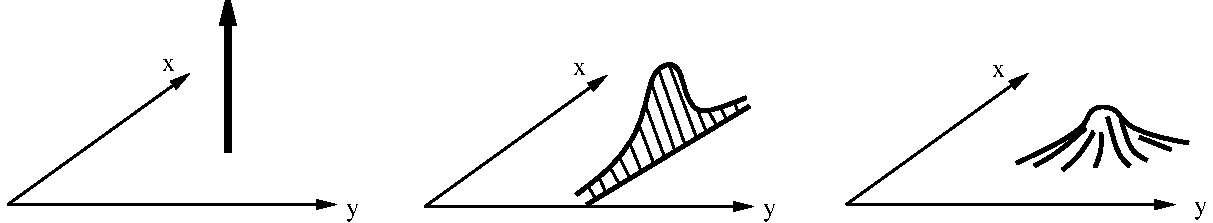
\includegraphics[width=0.95\textwidth]{txz/temperature}
\caption[temperature]{$(x,y)$平面内的温度分布。开始时为delta函数形状(左)。允许沿$x$方向但不沿$y$方向流动之后,热
量分希位于一片状区域内(中)。最后,允许热量沿$y$方向但不沿$x$方向流动,
得出同样的对称高斯分布的结果,其最终形状犹如热量同时沿$x$方向与$y$方向
流动,(右)}
\label{fig:txz/temperature}
\end{figure}


令人奇怪,在许多有关数值解的教科书中对全分离性没怎么介绍,这也许是由于不论是用
分裂法还是用全分离法求解,其加法与乘法的总次数是相同之故。但是,作为一个实际问
题,求解大数据量问题的计算时间并非简单随乘法次数而增高。当数据库不能整个输入于随
机存取器时(这差不多就是大数据量问题的定义),则分裂法的每一步骤都要求将数据库
加以转置。例如,从$(x,y)$的存储顺序转置成$(y,x)$的存储顺序。转置所要求的就不
是乘法,可是在许多情况下,转置所需时间却远超出整个计算所耗费的时间。所以,若进行
转置是不能避免时,至少应使它减少至实际允许的极小限度。有一些情况使得非在分裂法与
全分离法之间采取折中办法不可。例如,如果$\sigma$是$x$与$y$的一个缓慢变化的函数
时,就得如此,这时会发现,虽然$\sigma \partial^2/\partial x^2$并非严格可与
$\sigma \partial^2/\partial y^2$交换,可是却足够接近,因而在对数据进行转置
和转换至式\ref{eq:ex2.4.2b}之前,能够继续用式\ref{eq:ex2.4.2a}进行若干时间
步长的计算。以下要考虑的波场外推方程就是类似于这样一种但更具有地球物理意义的情况。第一个认识
到分裂法与全分离法概念在地震学中的意义是Brown(1983)。

\subsection{应用于横向速度变化情形}
\label{sec:2.4.4}
有一种情况:其中两个微分算子的不可交换性程度具有简单物理意义,且有明显有效之
地球物理应用,这种情形就是适用于非均匀介质的所谓单频15°波场外推方程。取时,
这种方程为
\begin{equation}
\frac{\partial U}{\partial z}=\{\frac{i\omega}{\bar{v}(z)}+i\omega
[\frac{1}{v(x,z)}-\frac{1}{\bar{v}(z)}]-\frac{\bar{v}(z)}{2i\omega}
\frac{\partial^2}{\partial x^2}\}U\\
=(retardation\quad + \quad thin\quad lens\quad +\quad diffraction)U
\label{eq:ex2.4.3}
\end{equation}
由式\ref{eq:ex2.4.3}可知,延迟项与薄透镜项可交换,且与自由空间绕射项可交换,但薄透镜项
与绕射项却彼此不能交换。看来,实际上最好是采用分裂法,用解析方法处理薄透镜项而用
Crank-Nicolson方法处理绕射项,这时,稳定性是有保证的,因为单独各个问题的稳定性
均已知。还有,解析解的精度也是引人入胜的一种特点。现在的问题是,这样两项在什么程
度上是可交换的?

这问题正好是幻灯投影仪的聚焦问题,调节聚焦旋钮就相当于调整薄透镜项,使之可与
自由空间绕射项相比。有的是小范围微调,没一个人能察觉出有任何差别;有的是大范围调
节,使后排座位的人不受错误聚焦的干扰。许多地球物理数据处理就是向下延拓数据,出现
在透镜项中的速度横向变化仅可已知到有限精度,要应用它就得利用外推办法来确定
$v(x)$。

对于很长的横向空间波长,各项是互换的,这时可忽略速度$v$之横向变动而进行绕射项
处理。波长较短时,则绕射项影响与透镜项影响必然是兼而有之。所以,现实问题并非仅仅
是计算的方便与不方便,而是数据精度与地下模型内速度可能变化范围之间的相互影响问题。

\subsection{应用于三维向下延拓}
\label{sec:2.4.5}

三维零炮检距反射地震资料的偏移算子是可利用Taylor级数展开至二阶的、即展开为
所谓的15°近似
\begin{equation}
[\frac{(-i\omega)^2}{v^2}-\frac{\partial^2}{\partial x^2}-\frac{\partial^2}{\partial y^2}]^{1/2}
\approx -\frac{i\omega}{v}-\frac{v}{-2i\omega}\frac{\partial^2}{\partial x^2}-\frac{v}{-2i\omega}\frac{\partial^2}{\partial y^2}
\label{eq:ex2.4.4}
\end{equation}
最普遍的情形为$v$是缓变化或$x$与义和$y$无关的情形,这时适用全分离法的条件。这是件好事,
因为它意味着我们可以利用普通的二维波场外推程序来处理三维情形,不论按照哪种顺序来
处理纵测线资料和联络测线上的资料都行。不过,当我们企图追求更高猜度时却碰到了
麻烦,要在Taylor级数展开时保留更多项数,很快就会遇到交错项$\partial^4 /\partial x^2\partial y^2$,像这样的
一项,既不能采用全分离法也无法采用分裂法。幸好,现代海上数据采集技术在沿垂直测线
方向迸行采集方面还相当粗糙,没必要采用超过15°的方程去进行沿垂直测线方向的处理。
Francis Muir曾经有一个好主意,用下式来表示平方根项:
\begin{equation}
[\frac{(-i\omega)^2}{v^2}-\frac{\partial^2}{\partial x^2}-\frac{\partial^2}{\partial y^2}]^{1/2}
\approx [\frac{(-i\omega)^2}{v^2}-\frac{\partial^2}{\partial x^2}]^{1/2}-\frac{v}{-2i\omega}\frac{\partial^2}{\partial y^2}
\label{eq:ex2.4.5}
\end{equation}
处理陆地资料时,为得到较好的近似,采用此式是必要的。在两个空间坐标轴中,至少沿其
中一个进行傅氏变换,将可解决计算问题。当介质速度并非横向变化如兜之快以致不能应用
傅氏变换时,这将是一科好办法。

\subsection{三维偏移的可分离性(Jakubowicz证法)}
\label{sec:2.4.6}

在运算条件下,三维偏移比二维偏移更难处理,因此,方便的是假设两次应用二维偏
移即可达到三维偏移的效果,一次沿$x$方向,另一次是沿$y$方向。前一节的论述也许
会使你相信,这样一种权宜的处理会使精度显著降低。其实,情况比可能想像的要好得多,
Jakubowicz与Levin(l985)等业已证明,真是出乎意外,这种权宜的处理方法在恒定速
度介质情形下是准确的。

这一点可这样解释:偏移不仅仅是由向下延拓所构成,它还涉及成像作用,即选出$t
=0$时的数据资料。从原理上说,首先是完成$x$方向与$y$方向的向下延拓,在那之后就适用成像条
件了。该种权宜处理过程共有四步:沿$x$方向的向下延拓、成像、沿$y$方向的向下延拓、最后
是第二次成像。这种权宜处理为什么能得出正确结果,看来似乎有点使人困惑不解,不过,
结论能成立却易于证实。

首先注意,式\ref{eq:ex2.4.6}代入式\ref{eq:ex2.4.7}即得出式\ref{eq:ex2.4.8}
\begin{equation}
t_1^2=t_0^2+(x-x_0)^2/v^2
\label{eq:ex2.4.6}
\end{equation}
\begin{equation}
t^2=t_1^2+(y-y_0)^2/v^2
\label{eq:ex2.4.7}
\end{equation}
\begin{equation}
t^2=t_0^2+(x-x_0)^2/v^2+(y-y_0)^2/v^2
\label{eq:ex2.4.8}
\end{equation}
式\ref{eq:ex2.4.8}代表到达某一任意的点散射体之旅行时间。在沿$y$轴(即$x$保持为常数时)进行记
录的二维勘测情形下,式\ref{eq:ex2.4.7}就是时距曲线方程.沿测线的双曲线时距曲线与侧反射
时距曲线不可能有什么区别,采用式\ref{eq:ex2.4.7}作二维偏移,使能量偏移至$t_1$,然后采用式\ref{eq:ex2.4.6}沿另一个方向进行偏移,将能量沿其余的路程偏移至$t_0$。,这样所得偏移结果同采
用式\ref{eq:ex2.4.8}进行很耗费时间的三维偏移处理所得结果是相同的。

Jakubowicz的证明则有点更为数学化,不过可解释其意义如下。首先注意,将式
\ref{eq:ex2.4.9}代入式\ref{eq:ex2.4.10}可得出式\ref{eq:ex2.4.11}
\begin{equation}
k_{\tau}^2=\omega^2-v^2k_x^2
\label{eq:ex2.4.9}
\end{equation}
\begin{equation}
k_z^2=\frac{k_\tau^2}{v^2}-k_y^2
\label{eq:ex2.4.10}
\end{equation}
\begin{equation}
k_z^2=\frac{\omega^2}{v^2}-k_x^2-k_y^2
\label{eq:ex2.4.11}
\end{equation}
沿$x$方向进行Stolt的二维偏移可看成是利用式\ref{eq:ex2.4.9}将旅行时间深度$t$变为赝深度(ps­eudodepth)$\tau$
的一种变换,沿$y$方向的第二个二维偏移可看成是利用式\ref{eq:ex2.4.10} 进行从赝
深度$\tau$至真深度$z$的一种变换,这种混合处理同描述三维偏移的式\ref{eq:ex2.4.11}是相同的。

Jakubowicz所得结论的有效性并不只限于证明本身。地球物理家也许除零炮检距情形
外还要对其他炮检距情形进行二维偏移(在第\ref{chap:offset}章中就讨论非零炮检距资料的偏移)。要是
作得顺利,所有反射能量均归位至零炮检距双曲线顶点,这时,交叉平面内的偏移就能像处
理零炮检距情形一样地处理,所以炮检距不成其为问题。但是,将所冇能量归位至零炮检距
双曲线的顶点究竟能不能顺利实现呢?

当地层速度像通常那样是与深度有关时,就出现了困难,这时Jakubowicz证明失效,因
而前述作权宜之计的三维方法也失效。利用二维勘测资料你要碰到一个问题:侧反射平面需
要有不同于沿垂直平面的偏移速度,传播至侧面的射线要取较长的路程才会达到地层深部的
高速介质,所以侧反射镰要较低的偏移速度。要是你真想用$v(z)$作三维偏移,你就应忘掉
分离法而用艰苦的方式完成它。不过,既然我们知道如何转置(见\ref{sec:1.6}节),因而艰苦的方
式其实也不见得非常艰苦。

\subsection{炮点与检波点空间内的可分离性}
\label{sec:2.4.7}

反射地震资料采集是在地面上完成的。人们想像能有这么一种资料出现,就好像是在
地层深部激发和记录到的一般,就是说,犹如炮点与检波点均深埋于地下一般。根据地面资
料可以人工作出这样的地下资料,首先将检波点向下外推,然后利用互换原理将震源与接
收点交换位置,最后再把地面震源(经互换原理处理之后,现在就是接收器了)向下外推。
第二种等价的处理办法是在炮点与检波点之间交错地按步长向下推进,这种办法在第3章中
将详尽研究,不过现在可用下式简单阐述其结论
\begin{equation}
\frac{\partial U}{\partial z}=\{
[\frac{(-i\omega)^2}{v(s)^2}-\frac{\partial^2}{\partial s^2}]^{1/2}+
[\frac{(-i\omega)^2}{v(g)^2}-\frac{\partial^2}{\partial g^2}]^{1/2}
\}U
\label{eq:ex2.4.12}
\end{equation}
这两种处理办法的等价性得出了一个数学上的推论,炮点坐标$s$与检波点坐标$g$均为独立变
量,所以式\ref{eq:ex2.4.12}中的两个平方根算子可互易。因此,采用分裂法可获得与采用全分离
法完全相同的结果。

\subsection{分裂概念与全分离概念的有效性}
\label{sec:2.4.8}
在有可能进行傅氏变换时,外推算子都是像$e^{ik_zz}$那样的复数。就复数$a$与$b$来说,$ab=ba$毫无疑问是成立的,因而,分裂法和全分离法总是能成立,但是只有根据更为一般化的讨
论才能给出证明。

假设始终未作傅氏变换,或者因为物性有某种空间变化而不可能作,这时,将前几节所述
之差分算子加以组合,用来构造外推算子。令$\mathbf{A}$与$\mathbf{B}$表示两个这类算子。例如,$\mathbf{A}$可以是一个
含有$x$方向之二阶差分算子的矩阵。视为矩阵时,微分算子的边界条件都位于矩阵各角上。
重要之点在于是否有关系式$\mathbf{AB}=\mathbf{BA}$,所以,问题显然不但涉及微分算子,而且还涉及边界条件。

短距离前向外推可以用算子$(\mathbf{I}+\mathbf{A}\Delta z)$完成。在二维问题中,把$\mathbf{A}$看成是一个四维矩
阵。为方便计,可将该四维矩阵的各项加以安排,成为一个超大型普通二维矩阵。隐式有限
差分计算曾得出像$(\mathbf{I}+\mathbf{A}\Delta z)/(\mathbf{I}-\mathbf{A}\Delta z)$这样的外推算子。令$\mathbf{P}$表示这样一个向量:该向
量的诸分量代表各种不同位置上的波场。以前已经知道,位置并不需限于$x$轴,而是也可以
分布于整个$(x,y)$平面。数值分析给我们提供一个矩阵算子,比如$\mathbf{A}$,它使我们能够迸行前
向投影,比如
\begin{equation*}
\mathbf{P}(z+\Delta z)=\mathbf{A_1}P(z)
\end{equation*}
$\mathbf{A}$有下标是表示算子可随$z$而变化。为间前推进一个步长,可再次应用该算子。比如
\begin{equation*}
\mathbf{P}(z+2\Delta z)=\mathbf{A_2}[\mathbf{A}_1P(z)]
\end{equation*}
从运算观点看,矩阵$\mathbf{A}$从未加以平方,但是从分析观点看,它确实是被平方了
\begin{equation*}
\mathbf{A}_2[\mathbf{A}_1\mathbf{P}(z)]=(\mathbf{A_2}\mathbf{A}_1)P(z)
\end{equation*}
要沿$z$轴向下推进若干距离,就多次应用该算子。取间隔$z_1-z_0$。,将它分成$N$个子区
间。由于有$N$个间隔,当达到了时间$z_1$时,每个子区间内与$1/N$成比例的误差将累积起来达
到不能令人接受的程度。另一方面,与$1/N^2$成比例的误差累积起来形成的总误差却仅与$1/N$
成比例。当增加子区间数时,这类误差将会消失。

为证明分裂法的有效性,现取$\Delta z=(z_1-z_0)/N$。可以看到,算子$\mathbf{I}+(\mathbf{A}+\mathbf{B})\Delta z$不同于算子$(\mathbf{I}+\mathbf{A}\Delta z)(\mathbf{I}+\mathbf{B}\Delta z)$,后者大体是与$\Delta z^2$或者$1/N^2$成比例的,所以,在子区间
数非常大的极限情形下,误差就消失了。

全分离概念的有效性是非常容易证实的。互易性就在于关系$\mathbf{AB}=
\mathbf{BA}$是否成立,对于标
量,互易性恒成立;采用有限差分时,问题就在于两个矩阵是否可互易。取$\mathbf{A}$与$\mathbf{B}$为微分算
子,藉助于所有可能的波场$P$来定义互易性,这时,如果$\mathbf{AB}P=\mathbf{BA}P$,则$\mathbf{A}$与$\mathbf{B}$就是可互易
的。

代表$\partial P/\partial z$的算子将取为$\mathbf{A}+\mathbf{B}$,采用分裂法时最简单的数值积分格式为
\begin{equation}
P(z_0+\Delta z)=(\mathbf{I}+\mathbf{A}\Delta z)(\mathbf{I}+\mathbf{B}\Delta z)P(z_0)
\label{eq:ex2.4.13}
\end{equation}
在许多步长内应用式\ref{eq:ex2.4.13},得出许多算子之乘积,给算子$\mathbf{A}$与$\mathbf{B}$加下标$i$,用以表示它
们随$z$而变化的可能性,于是
\begin{equation}
P(z_i)=\prod_{i=1}^N[(\mathbf{I}+\mathbf{A}\Delta z)(\mathbf{I}+\mathbf{B}\Delta z)]P(z_0)
\label{eq:ex2.4.14}
\end{equation}
